\subsection{Objectives}
\begin{itemize}
\item Create an Oracle User for yourself.
\item Gain access to the Oracle system.
\item Meet the APEX Oracle environment 
\item Practice entering and running simple statements (without understanding them in detail)
\item Gain an exposure to error messages.
\end{itemize}
\subsection{Creating your User in ORACLE }
All students must register as an Oracle User.  For this you will need:

\begin{itemize}
\item your Student Number
\item your personal details
\end{itemize}
Start https://dbutils.shu.ac.uk/oracleutility  or from the Start menu



\begin{center}
  
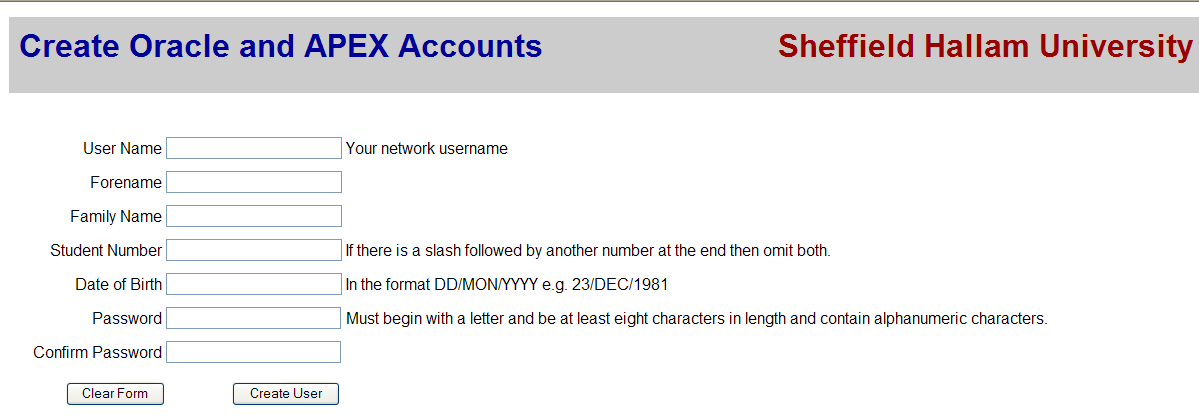
\includegraphics[width=13.201cm,height=4.574cm]{images/img (3).png}

\end{center}
\begin{center}
\begin{minipage}{4.177cm}
Enter your Log-in Id, Name and Student Number
\end{minipage}
\end{center}


\begin{center}
\begin{minipage}{4.177cm}
The format for Date of Birth is

dd/mmm/yyyy, e.g. 01/JAN/1990
\end{minipage}
\end{center}


\begin{center}
\begin{minipage}{14.441cm}
Choose a password (that you will remember!). The password rules:

\begin{itemize}
\item eight characters in length
\item start with a letter
\item the remainder may be letters or numbers
\item Oracle passwords are NOT case sensitive
\end{itemize}
\end{minipage}
\end{center}
Click the 'Create User' button, and wait. Interrupting the process can corrupt your Oracle details and you may not be able to re-run the process. If successful you now have a personal and private Oracle environment and two accounts: for Oracle, the DBMS, and for APEX, the Web front-end. Both use the same username and password. The database has been populated with the three Personnel Systems tables that we will use throughout the semester.

If you did not get an account, check that the format of your entries is correct. Does the University know you by different personal details? If your name, or your date of birth, is recorded by the University with a typo, enter it here with

\begin{center}
  

\includegraphics[width=1.06cm,height=0.903cm]{images/img (2).png}

\end{center}
the same typo. If you still don't seem to get an account, ask for help -- we'll ensure you do.

\clearpage 
\subsection{Starting Oracle}
Once you have your account, access the APEX facility via  one of the following paths:

Start Menu/Programs/Specialist Applications/Oracle/Application Express Login/

or:

http://homepages.shu.ac.uk:7777/pls/apex

You will be prompted for your Oracle User Code and Workspace (use your username for both) and your Oracle Password.



\begin{center}
  
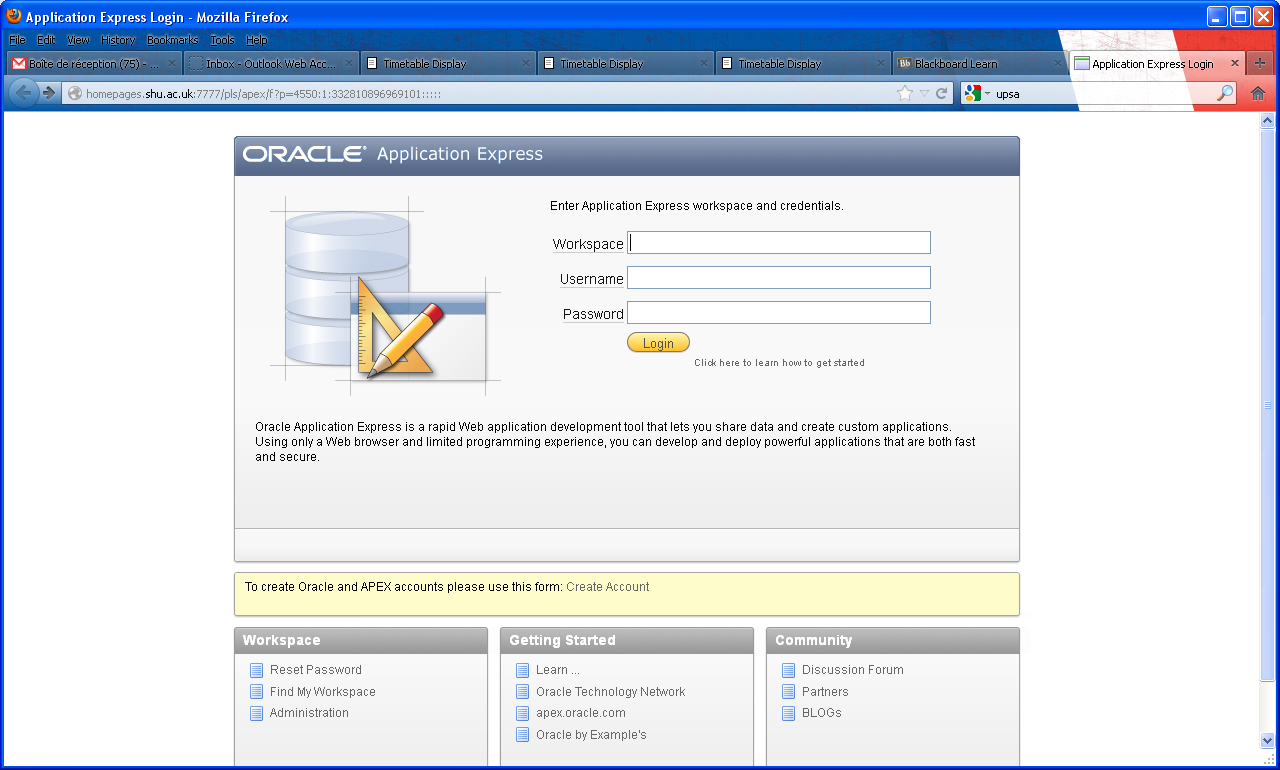
\includegraphics[width=9.479cm,height=3.41cm]{images/img (4).png}

\end{center}
\begin{center}
\begin{minipage}{4.092cm}
Workspace and Username are the same, enter it twice
\end{minipage}
\end{center}
Oracle will present you with APEX web interface.

\begin{center}
\begin{minipage}{3.958cm}
Select 

SQL Workshop
\end{minipage}
\end{center}


\begin{center}
  
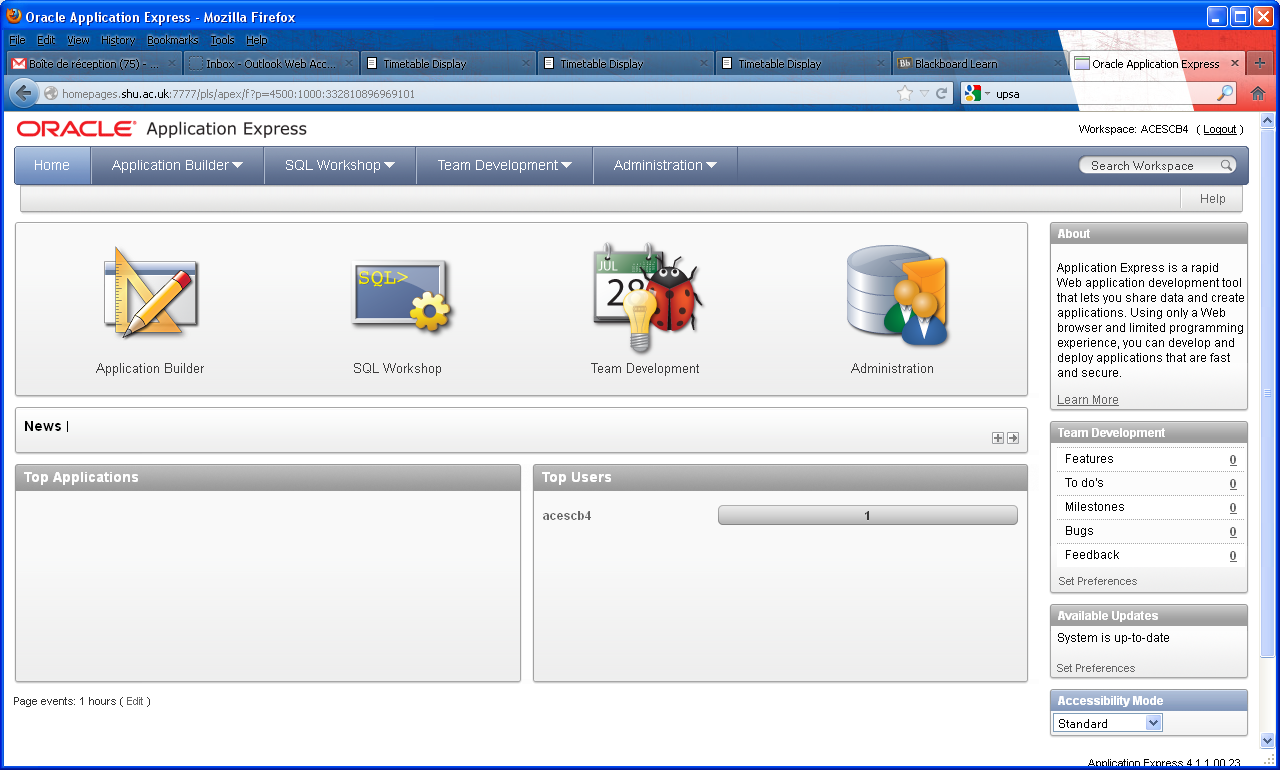
\includegraphics[width=13.028cm,height=3.478cm]{images/img (5).png}

\end{center}
The screen now shows four features. During this module you will use the first three:



\begin{center}
  
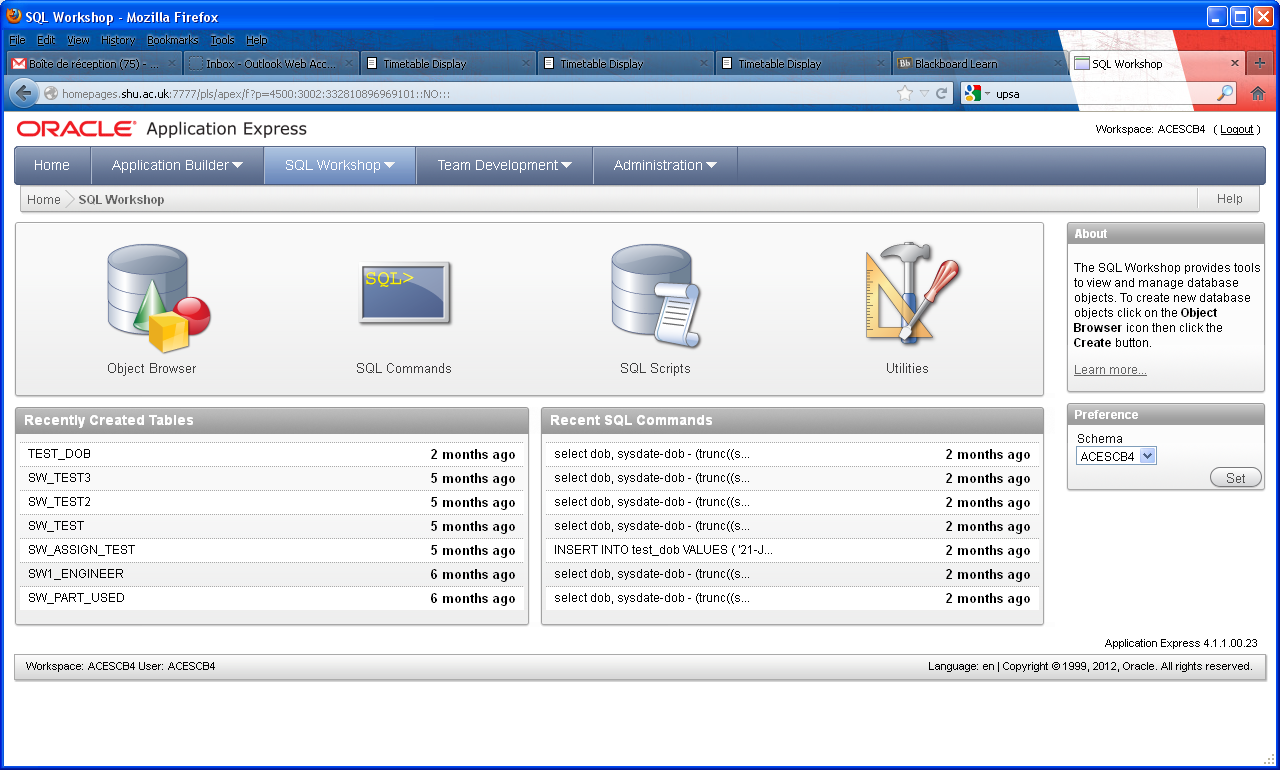
\includegraphics[width=13.162cm,height=2.436cm]{images/img (6).png}

\end{center}


\begin{center}
\begin{minipage}{6.368cm}
SQL Scripts:

save commands to execute (or re-execute) later, or save multiple commands to execute in batch.
\end{minipage}
\end{center}
\begin{center}
\begin{minipage}{4.189cm}
SQL Commands: 

type SQL that is immediately executed;
\end{minipage}
\end{center}
\begin{center}
\begin{minipage}{3.981cm}
Object Browser:

explore the tables and other objects forming your database
\end{minipage}
\end{center}
By the end of this Lab session you will have tried all three of them.

Select the SQL Commands feature. A two part screen will be displayed.

\begin{center}
  
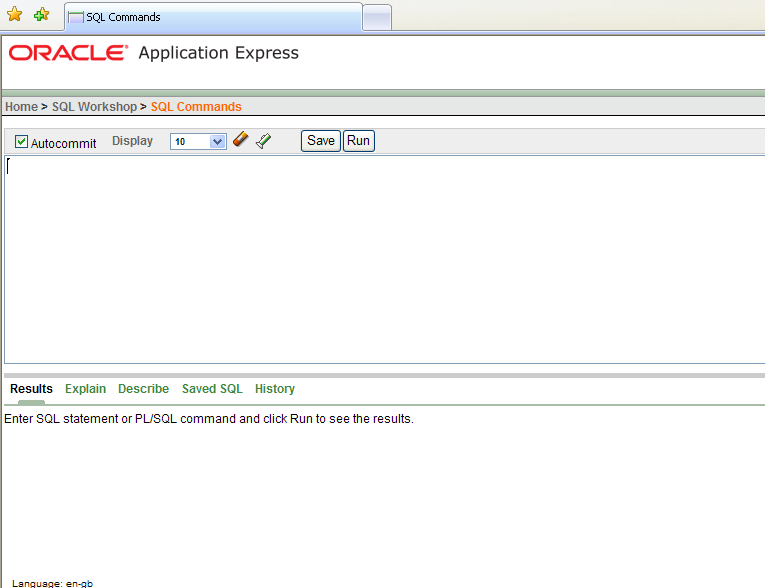
\includegraphics[width=13.728cm,height=10.4cm]{images/img (7).png}

\end{center}


\begin{center}
\begin{minipage}{4.584cm}
Save statements to check or re-run later
\end{minipage}
\end{center}
\begin{center}
\begin{minipage}{4.246cm}
Display option:  controls how many results are displayed (check it: are some rows not displayed?)
\end{minipage}
\end{center}


\begin{center}
\begin{minipage}{2.789cm}
Clear Command (eraser); remove the current statement

\end{minipage}
\end{center}
\begin{center}
\begin{minipage}{4.706cm}
Top section: enter your statements here.
\end{minipage}
\end{center}


\begin{center}
\begin{minipage}{4.944cm}
Lower section: the results of running that statement.
\end{minipage}
\end{center}
You are now ready to issue SQL statements.

\subsection[First steps]{First steps}
\begin{itemize}
\item 
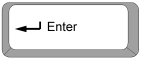
\includegraphics[width=1.63cm,height=0.683cm]{images/img (8).png}
  is the Enter key on the keyboard 
\end{itemize}
\begin{itemize}
\item After entering each statement click the 
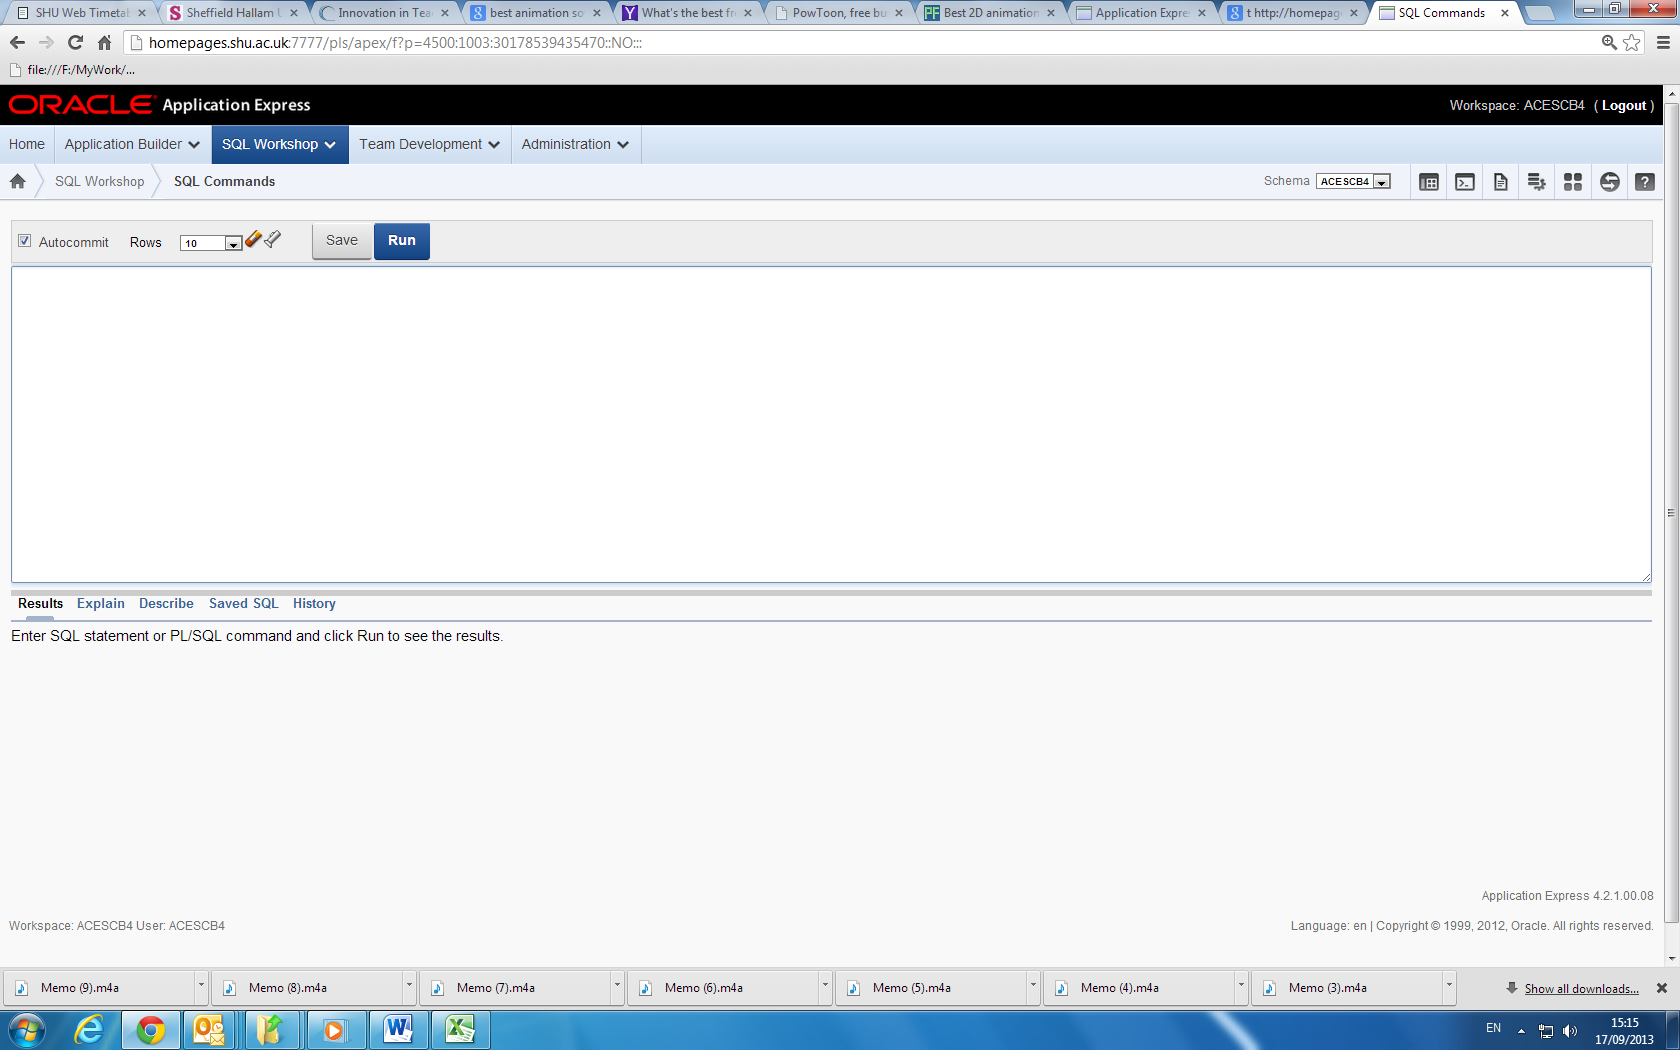
\includegraphics[width=0.947cm,height=0.607cm]{images/img (9).png}
  button. 
\end{itemize}
\begin{itemize}
\item Study the results and, for each group of statements, write down your conclusions.
\end{itemize}
\begin{itemize}
\item Now type in the following commands or statements exactly as presented
\end{itemize}
Try this:

SELECT  *  from EMP; 
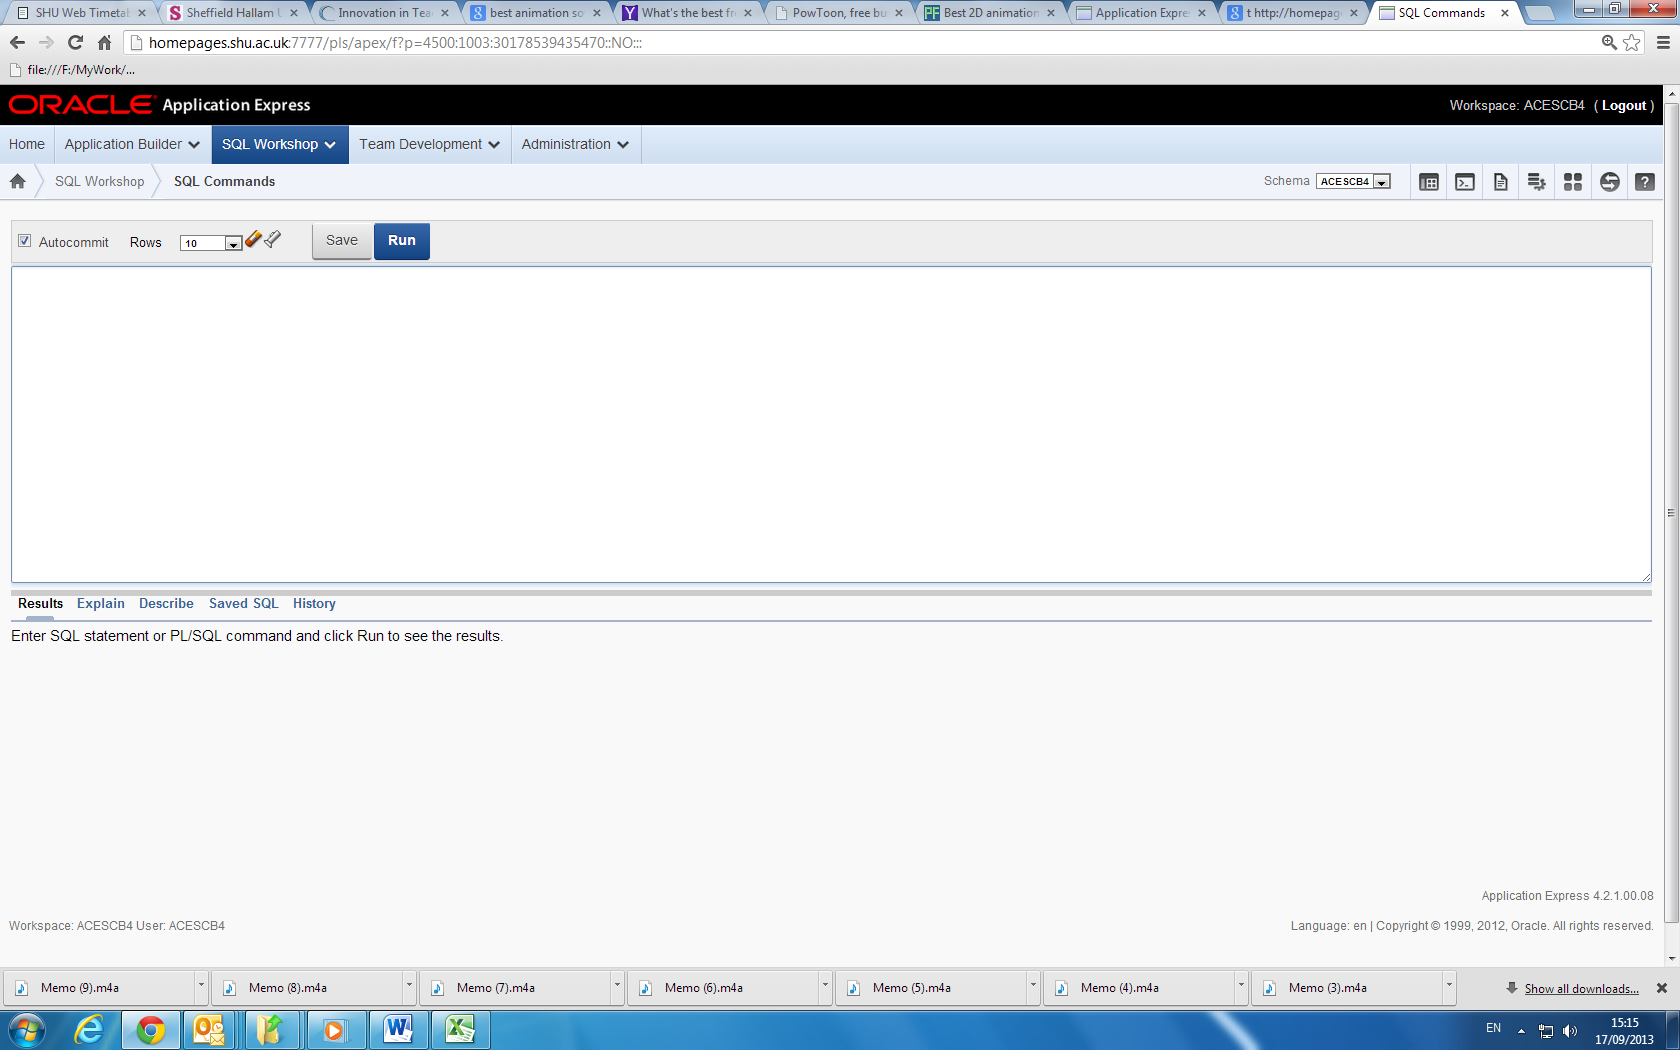
\includegraphics[width=0.947cm,height=0.607cm]{images/img (9).png}
 

The command should return the contents of the EMP table (example result over the page).

Oracle (helpfully?) makes the semi-colon optional for single statements, though it is the standard. These rules vary between database vendors: the {\textquotedbl}safe{\textquotedbl} approach is to follow the standard, and always use a semi-colon.

\begin{center}
  

\includegraphics[width=1.058cm,height=0.903cm]{images/img (2).png}

\end{center}
   
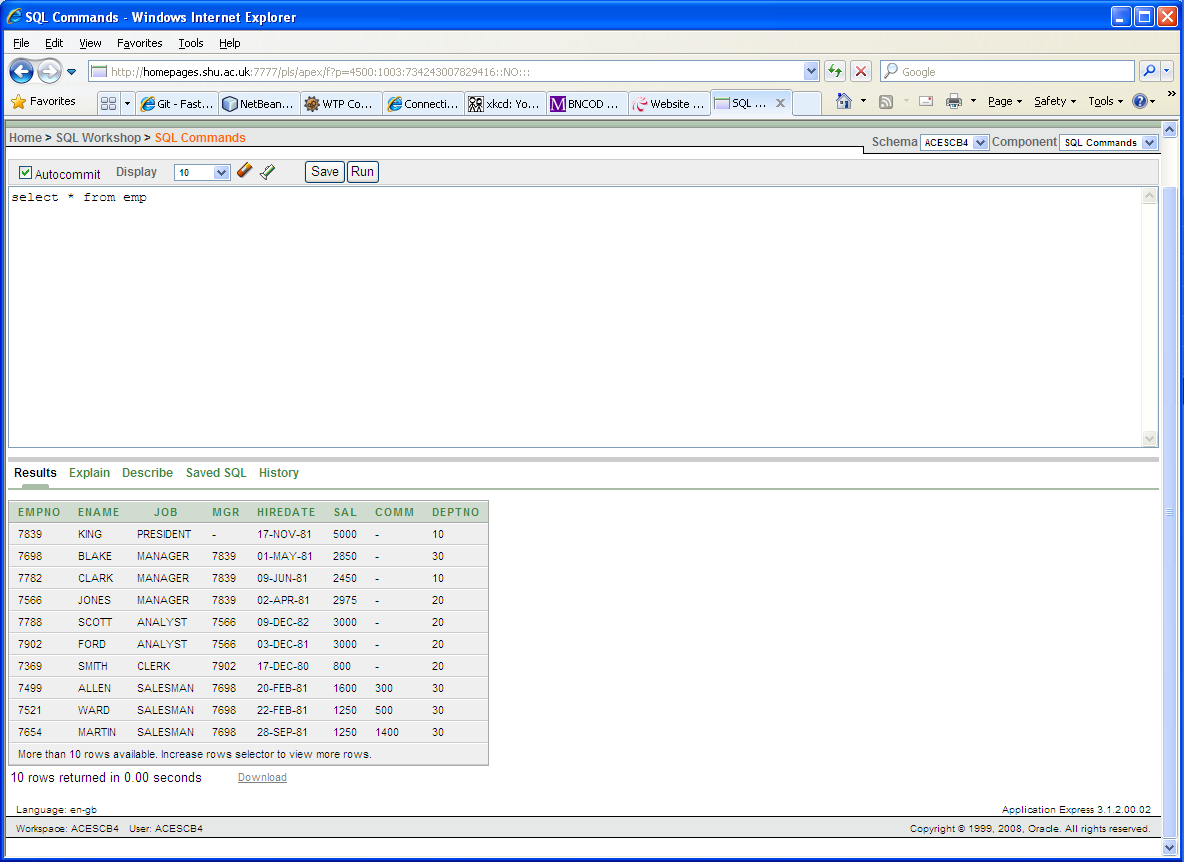
\includegraphics[width=14.785cm,height=8.871cm]{images/img (10).png}
 

Now try these alternatives, one at a time. Clear the upper part of the screen before entering each one:

Do lower case commands work? Clear the last command and type

select  *  from emp; 
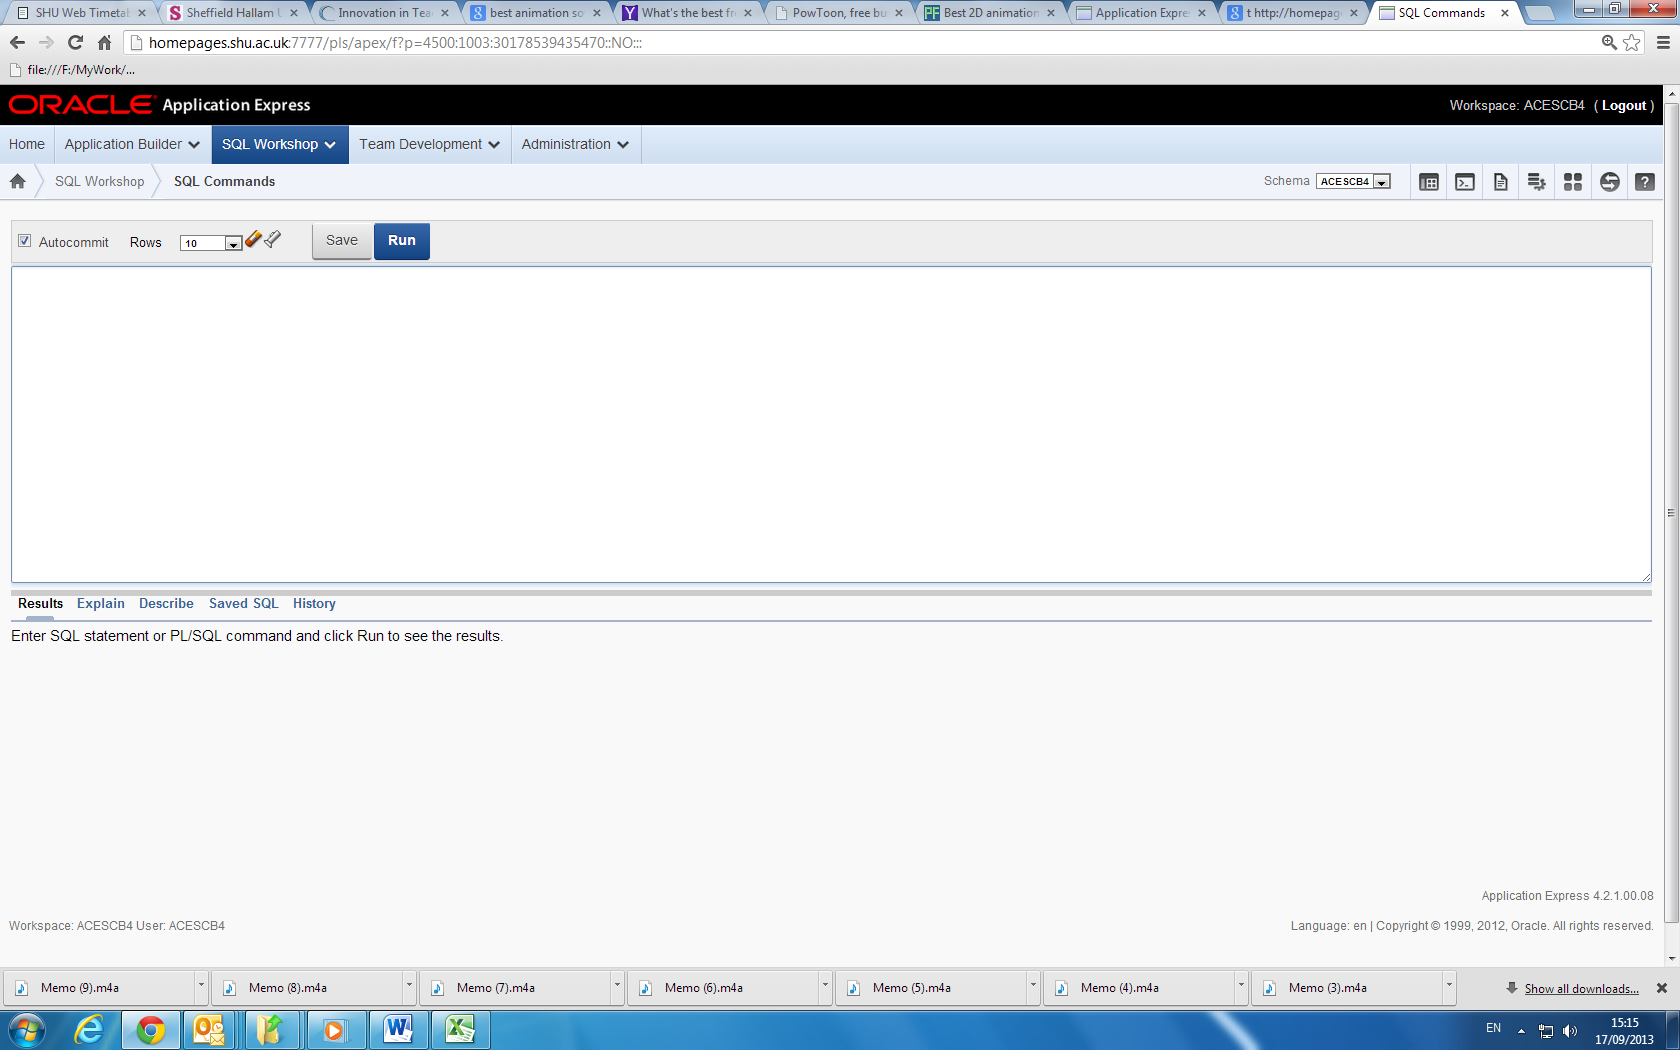
\includegraphics[width=0.947cm,height=0.607cm]{images/img (9).png}
 

and (you don't have to retype, edit the previous command):

Select  *  from EmP; 
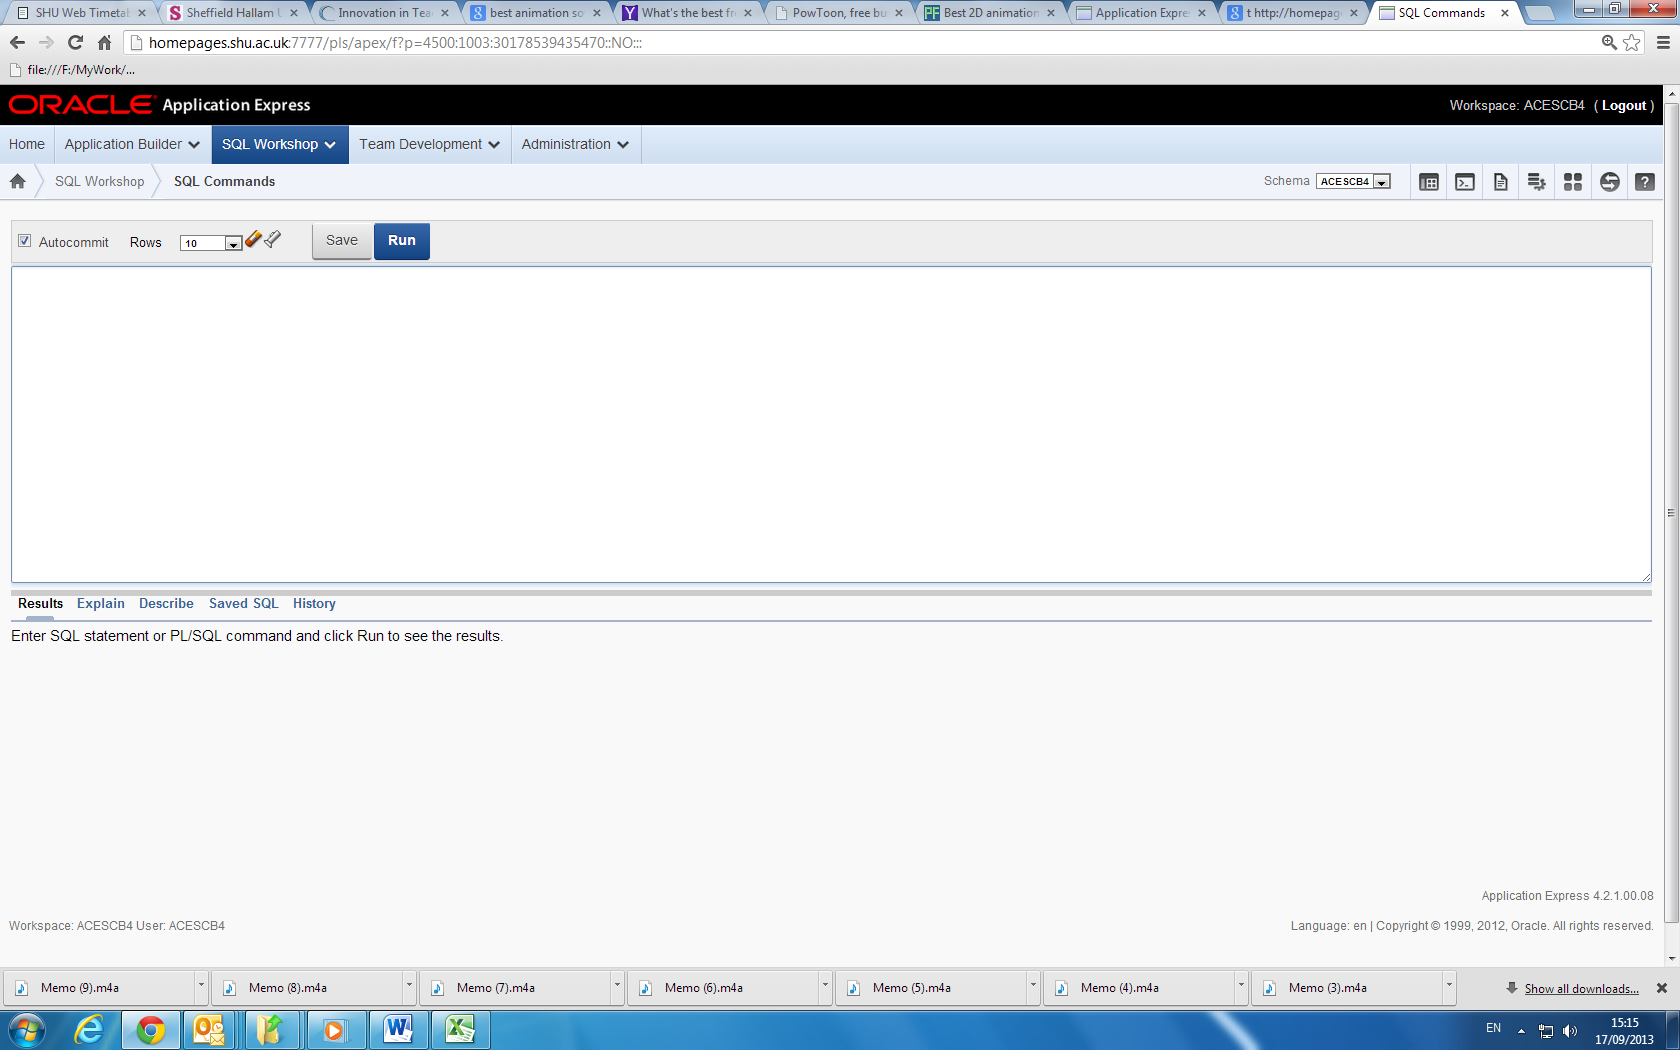
\includegraphics[width=0.947cm,height=0.607cm]{images/img (9).png}
 

Is white space -- new lines, spaces -- allowed in commands? Try

select  *  from  
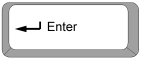
\includegraphics[width=1.63cm,height=0.683cm]{images/img (8).png}
 

 emp; 
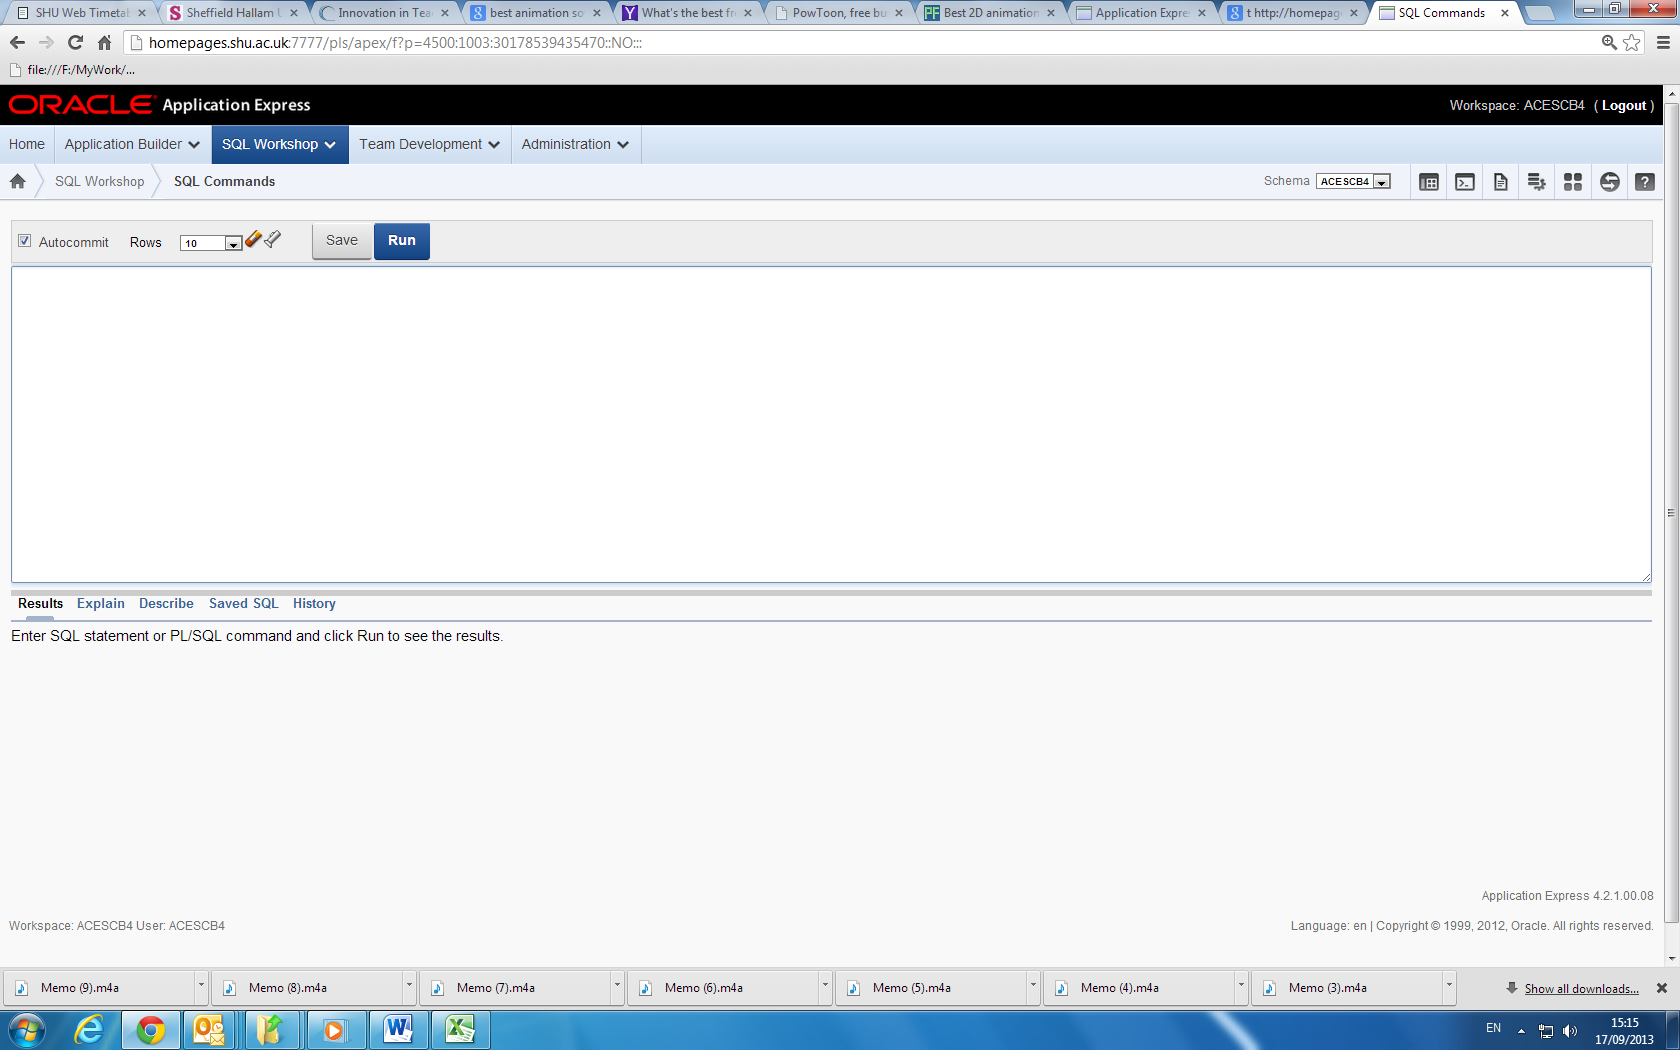
\includegraphics[width=0.947cm,height=0.607cm]{images/img (9).png}
 

You may wish to discuss your conclusions with a colleague. Keep notes of what you find out - about the use of case, of white space, any errors you have to deal with and how you resolve them.



\begin{center}
  

\includegraphics[width=1.048cm,height=0.903cm]{images/img (2).png}

\end{center}
Scribbling on this workbook is definitely allowed!

Oracle techniques

Note: the techniques that follow are ORACLE-specific, and wouldn't work as such with other DB management systems.

Now enter all of the following before pressing the Run button:

\ \ select * from emp;  
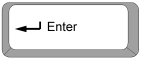
\includegraphics[width=1.63cm,height=0.683cm]{images/img (8).png}
 

\ \ select * from dept;

\begin{center}
  
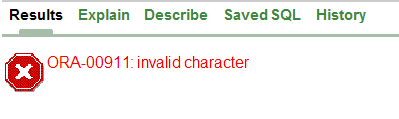
\includegraphics[width=10.137cm,height=3.044cm]{images/img (11).png}

\end{center}
You now have an error message.  Unfortunately the message is unhelpful. SQL statements are correctly separated with a ; (semi-colon), but  from the SQL workshop, Oracle cannot run both statements in succession. One solution is to first highlight the statement you wish to run:

Highlight the first 'select * from emp;' and press the run button.  You should recognise the results.

\subsection{Checking the objects available}


\begin{center}
  
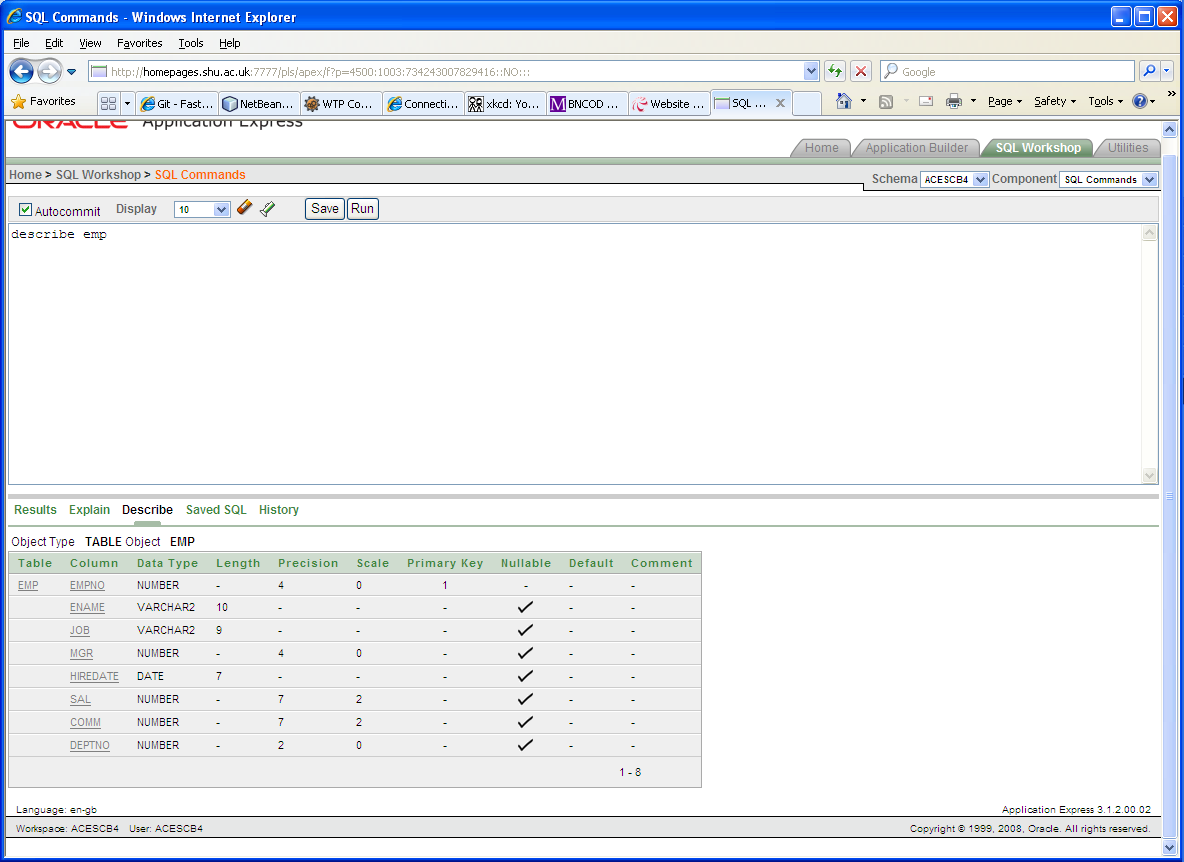
\includegraphics[width=9.35cm,height=4.944cm]{images/img (12).png}

\end{center}
Try this:

\emph{DESCRIBE table\_name;}

is a useful command. It displays a table definition, e.g.

\ \ DESCRIBE\ \ EMP;

gives the result on the right.



\begin{center}
  
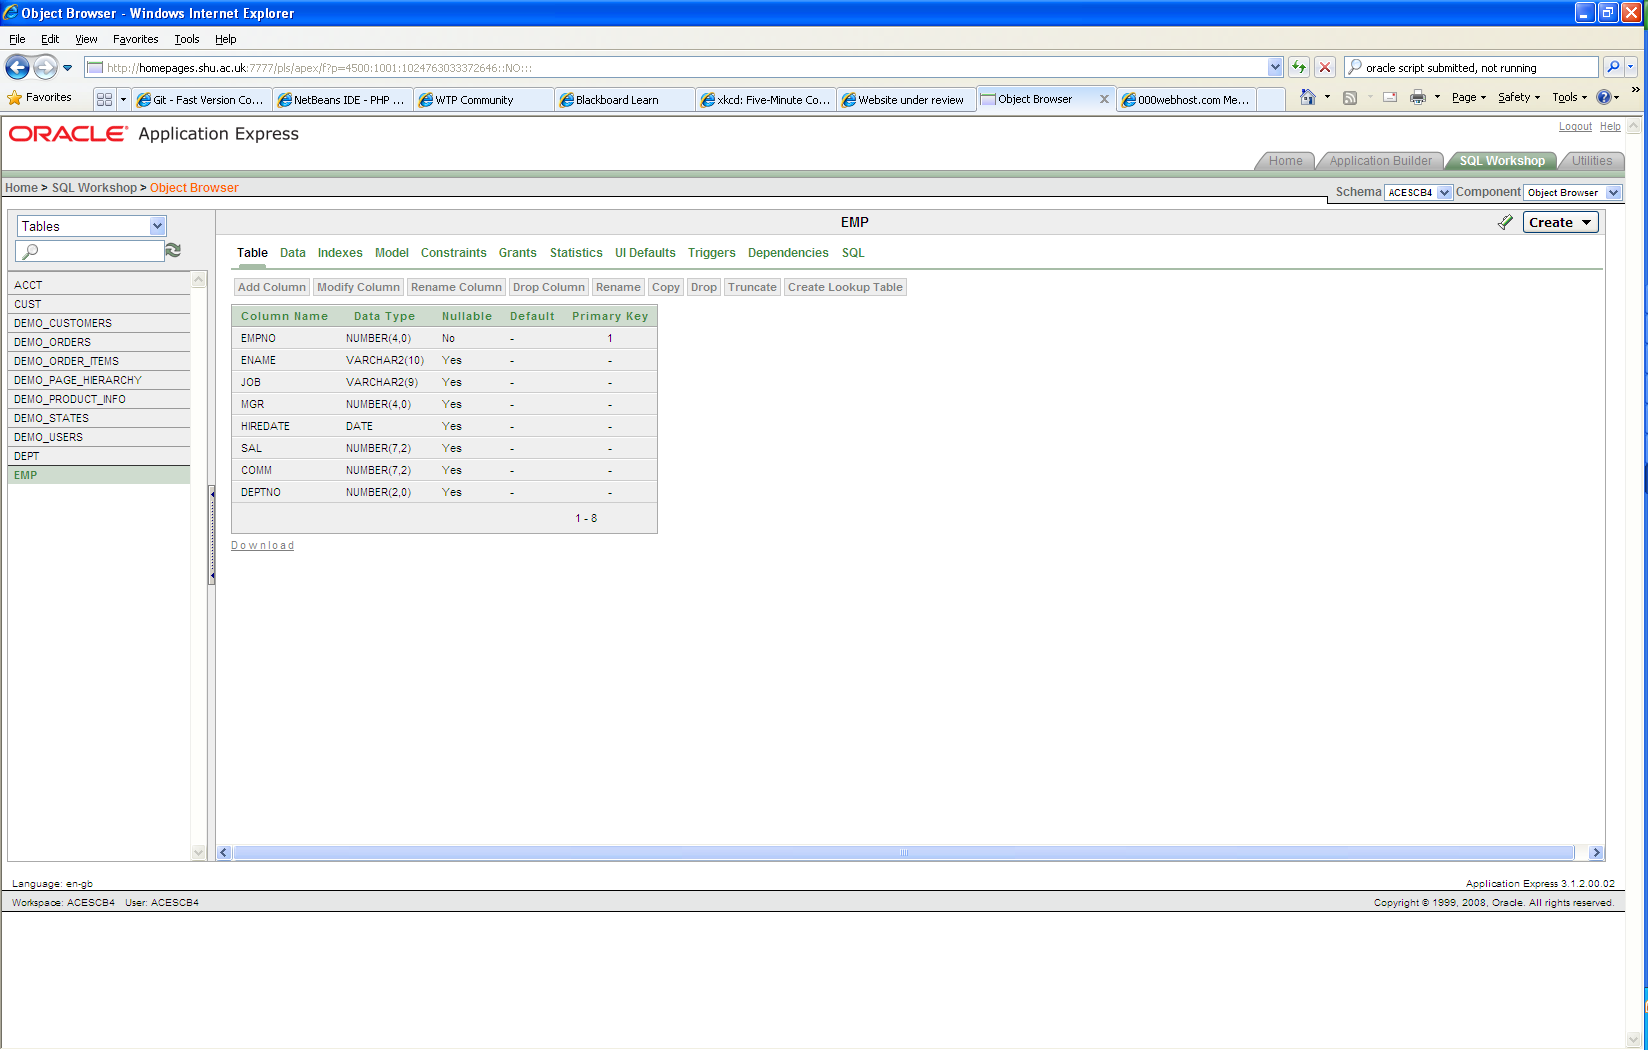
\includegraphics[width=8.751cm,height=5.309cm]{images/img (13).png}

\end{center}
Now move to the 'Home{\textgreater}SQL Workshop' screen and select the 'Object browser' feature. It shows details of all the tables, views and other objects that exist within your Oracle environment. 

Finally, the following gives details of the tables and views you currently own:

SELECT  *  from TAB;

ORACLE has a data dictionary that holds details of the database definition and its environment.  The query returns those details, as if {\textquotedbl}TAB{\textquotedbl} was a table of your tables.

About the exercises

\begin{itemize}
\item Do not rush; take time to understand what is happening.
\item When you get errors, study your statement(s) and the data (or error messages!) to determine a solution; do NOT get into a 'hacking' mode.
\item Think what results you would expect from the statement(s) you are issuing and carefully check them against the generated result.
\item Note your solutions. You can use this workbook for the purpose, or save scripts (one script for each section of the workbook?).  You will find it useful to refer back to earlier work.
\item Discuss problems and uncertainties with your tutor, they are there to help.
\item Maintain progress. Each section is very dependent on understanding previous ones.
\end{itemize}
We hope you enjoy the experience.

\subsection{About notation to describe SQL syntax}
SQL statements are made of multiple clauses. As they are sometimes difficult to explain, this book describes the different combinations of keywords using some special characters.

\begin{itemize}
\item Anything that needs to be replace is in italics; example:
\end{itemize}
\ \ SELECT * FROM table

table is actually not the word to type, but a word to substitute replace by the name of the actual table you want.

\begin{itemize}
\item Optional elements are included in [square brackets] [ ], are optional. Ffor example:
\end{itemize}
\ \   \ \ SELECT * FROM table [ WHERE Criteria ] ;

cWhich indicates that the section {}``WHERE Criteria{}'' is ould be either:\ \ SELECT * FROM table ;

\ \ or\ \ \ \ \ \ SELECT * FROM table WHERE Criteria ;



\begin{center}
  

\includegraphics[width=1.048cm,height=0.903cm]{images/img (2).png}

\end{center}
in option.

Don't type the square brackets! The same is true of the other signs below the other notation signs below.

\begin{itemize}
\item Optional repetition is marked using ... as follows:
\end{itemize}
\ \   SELECT col1 [ , col2 ... ]  FROM table  [ WHERE Criteria ] ;

This means that there can be one or more columns.

\begin{itemize}
\item Finally, we use and the vertical bar {\textbar} (also called the pipe symbol) and if need be, braces \{ \} to denote alternatives:
\end{itemize}
 SELECT \{ * {\textbar} columns-list \} FROM table ;

Means that you can use either a list of columns, or the * with this statement.

\clearpage